\subsection{Random Forest}

\subsubsection{Mô hình cho tập dữ liệu chỉ bao gồm các quan sát có cột "emailtotal" không phải giá trị null}

\begin{enumerate}[label=(\alph*)]
    \item Đầu vào mô hình là vector thu được từ phân tích thành phần chính sử dụng thuật toán PCA
    
    Ta có bảng kết quả huấn luyện mô hình:

    \begin{python}
                    precision    recall  f1-score   support

   Keeping house       0.00      0.00      0.00        58
           Other       0.00      0.00      0.00         8
         Retired       0.00      0.00      0.00       109
          School       0.00      0.00      0.00        14
Temp not working       0.00      0.00      0.00        15
Unempl, laid off       0.00      0.00      0.00        25
Working fulltime       0.53      1.00      0.69       351
Working parttime       0.00      0.00      0.00        80

        accuracy                           0.53       660
       macro avg       0.07      0.12      0.09       660
    weighted avg       0.28      0.53      0.37       660
    \end{python}

    và ma trận nhầm lẫn:

    \begin{figure}[H]
        \centering
        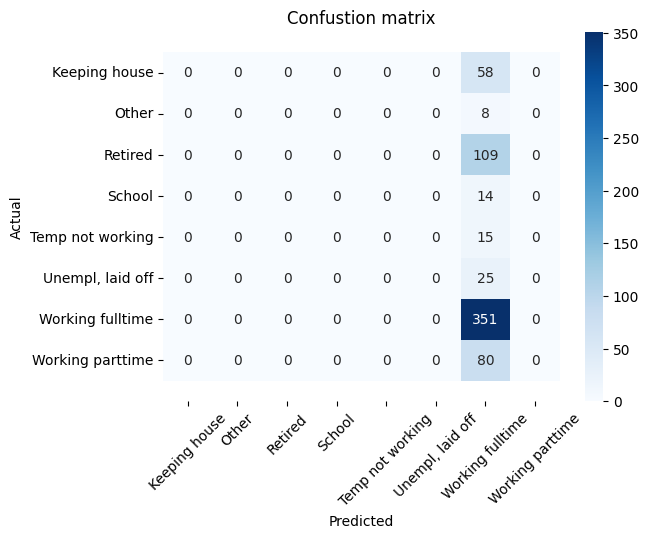
\includegraphics[width=0.6\textwidth]{figures/Thanh/Models/Random_Forest/Non_null_models_confusion_matrix_Random_Forest_PCA_features.png}
        \caption{Ma trận nhầm lẫn của mô hình Random Forest với vector đầu vào là vector thu được từ phân tích thành phần chính sử dụng thuật toán PCA}
        \label{fig:Non_null_models_confusion_matrix_Random_Forest_PCA_features}
    \end{figure}

    Ta nhận thấy kết quả không tốt hoàn toàn giống hệt với kết quả của mô hình Logistic Regression.
    Mô hình dự đoán tất cả các quan sát vào lớp làm việc toàn thời gian.
    Lý do là vì từ phần phân tích dữ liệu, ta thấy phân phối của các thành phần chính tương ứng với các nhóm trong cột wrkstat gần như cùng hình dạng, trộn lẫn vào nhau.
    Mô hình sẽ khó phân biệt được quan sát nào thuộc lớp nào.
    Trong quá trình học, mô hình biết số quan sát thuộc lớp làm việc toàn thời gian có số lượng nhiều nhất.
    Vì do phân phối của các lớp gần giống nhau hoàn toàn, mô hình sẽ học bằng cách là dự đoán các tất cả các quan sát đến vào cùng một lớp.
    Khi dự đoán như vậy để hàm cross entropy trên dữ liệu là nhỏ nhất, mô hình buộc phải chọn dự đoán tất cả các quan sát có số lượng nhiều nhất mà mô hình đã biết từ tập huấn luyện.

    Ta sẽ phân tích ngược trở lại trọng số của các tham số tương ứng với các đặc trưng của vector ban đầu từ các tham số ứng với các đặc trưng của các thành phần chính:

    \begin{figure}[H]
        \centering
        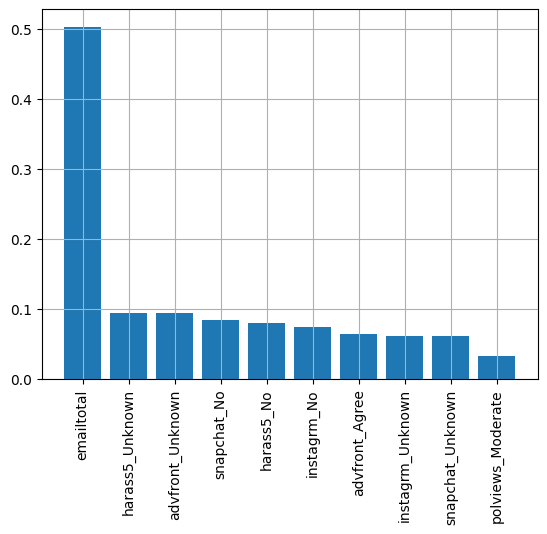
\includegraphics[width=0.6\textwidth]{figures/Thanh/Models/Random_Forest/Non_null_models_Feature_Importance_Random_Forest_PCA_features.png}
        \caption{Biểu đồ cột sắp xếp độ lớn giảm dần (trị tuyệt đối) tham số của các đặc trưng (mô hình với vector đầu vào là vector được phân tích thành phần chính sử dụng thuật toán PCA)}
        \label{fig:Non_null_models_Feature_Importance_Random_Forest_PCA_features}
    \end{figure}
    
    Ta có biểu đồ cột sắp xếp độ lớn giảm dần (trị tuyệt đối) tham số của các đặc trưng thể hiện ở hình \ref{fig:Non_null_models_Feature_Importance_Random_Forest_PCA_features}.
    Ta nhận thấy các cột có trọng số lớn và ảnh hưởng nhiều tới các các nhãn đầu ra là emailtotal, harass5\_Unknown.
    Hai đặc trưng này có tần suất xuất hiện lớn trong tập dữ liệu.

    \item Vector đầu vào là vector gốc ban đầu
    
    Ta có bảng kết quả huấn luyện mô hình:

    \begin{python}
                    precision    recall  f1-score   support

   Keeping house       0.00      0.00      0.00        58
           Other       0.00      0.00      0.00         8
         Retired       0.00      0.00      0.00       109
          School       0.00      0.00      0.00        14
Temp not working       0.00      0.00      0.00        15
Unempl, laid off       0.00      0.00      0.00        25
Working fulltime       0.53      1.00      0.69       351
Working parttime       0.00      0.00      0.00        80

        accuracy                           0.53       660
       macro avg       0.07      0.12      0.09       660
    weighted avg       0.28      0.53      0.37       660

    \end{python}

    và ma trận nhầm lẫn

    \begin{figure}[H]
        \centering
        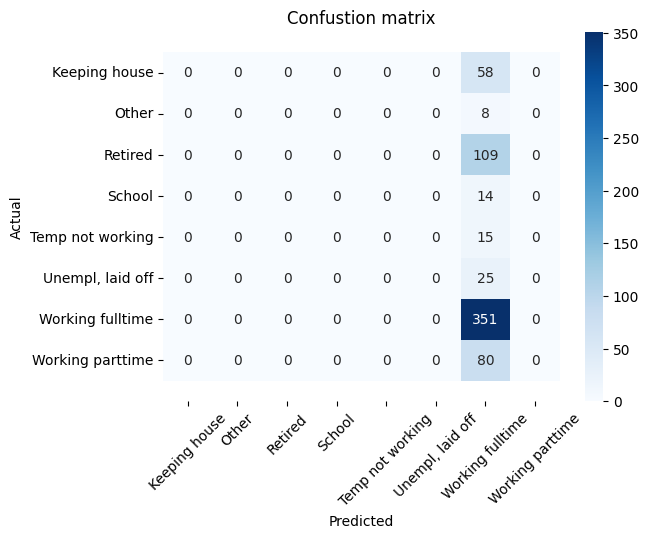
\includegraphics[width=0.6\textwidth]{figures/Thanh/Models/Random_Forest/Non_null_models_confusion_matrix_Random_Forest_PCA_features.png}
        \caption{Ma trận nhầm lẫn của mô hình Random Forest khi vector đầu vào là vector gốc ban đầu}
        \label{fig:Non_null_models_confusion_matrix_Random_Forest_PCA_features}
    \end{figure}
    
    Ta nhận thấy kết quả phân loại của mô hình hoàn toàn giống trường hợp đầu vào mô hình là vector được phân tích thành phần chính sử dụng thuật toán PCA.

    Ta sẽ phân tích ngược trở lại trọng số của các tham số tương ứng với các đặc trưng của vector ban đầu từ các tham số ứng với các đặc trưng:

    \begin{figure}[H]
        \centering
        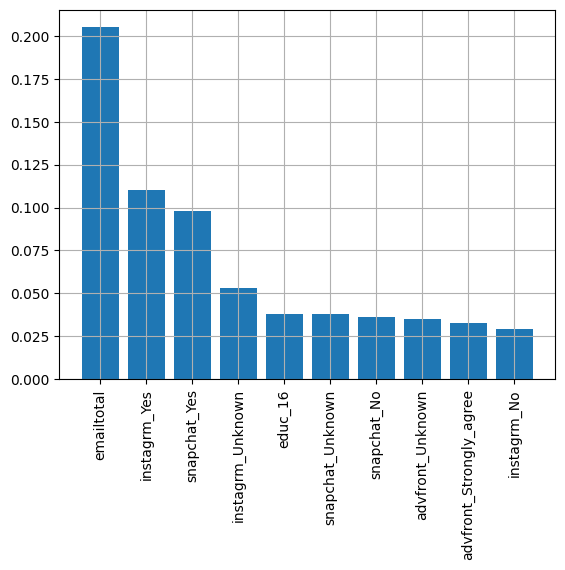
\includegraphics[width=0.6\textwidth]{figures/Thanh/Models/Random_Forest/Non_null_models_Feature_Importance_Random_Forest_original_features.png}
        \caption{Biểu đồ cột sắp xếp độ lớn giảm dần (trị tuyệt đối) tham số của các đặc trưng (mô hình với vector đầu vào là vector gốc ban đầu)}
        \label{fig:Non_null_models_Feature_Importance_Random_Forest_original_features}
    \end{figure}

    Ta có biểu đồ cột sắp xếp độ lớn giảm dần (trị tuyệt đối) tham số của các đặc trưng thể hiện ở hình \ref{fig:Non_null_models_Feature_Importance_Random_Forest_original_features}.
    Ta nhận thấy các đặc trưng có trọng số lớn tương ứng là snapchat\_Yes, instagrm\_Yes đa số là các đặc trưng ít xuất hiện trong tập dữ liệu.
    emailtotal có trọng số lớn nhất.
\end{enumerate}